\hypertarget{chap:intro}{\chapter{Introduction}}
\section{Overview}
\subsection{Sentiment Analysis and its applications}
\subsubsection{Definition}
In a nutshell, sentiment analysis is to determine whether the opinion about a specific product, event, organization is positive or negative. It is also known as opinion mining due to the sentiment was derived from opinions of the speaker.

The main objective of sentiment analysis is given document $d$ define as quintuples \cite{liu2012sentiment}:
\[ ( e_{i}, a_{ij}, s_{ijkl}, h_{k}, t_{l} ) \]
 Where:
\begin{itemize}
	\item $e_{i}$: entity i (entity extraction and categorization)
	\item $a_{ij}$: aspect j of entity i (entity extraction and categorization)
	\item $h_{k}$: holder k (opinion holder extraction and categorization)
	\item $t_{l}$: time l (time extraction and standardization)
	\item $s_{ijkl}$: opinion of holder k about aspect j of entity i at time l (aspect sentiment classification)
\end{itemize}


\subsubsection{Different levels in sentiment analysis}
\paragraph{Document-level}
Document-level sentiment analysis is a text classification problem. The system was given a document $d$ and classifies whether the overall opinion was positive, negative. The document can be a reviews of a movie. For example, Pang and Lee ~\cite{pang2002thumbs} perform document-level sentiment analysis on IMDB movies review data. Document-level sentiment analysis assumes that whole document gives an opinion toward one entity and does not apply to documents containing multiple entity ~\cite{liu2012sentiment}.

\paragraph{Sentence-level}\label{sec:sent-level}
Sentence-level sentiment analysis is to determine whether a sentence expressed positive or negative. Similar to document-level sentiment analysis, a sentence is assumed only contain opinion toward one entity (a single movie) ~\cite{liu2012sentiment}.
In this thesis, we focus our study on sentence-level sentiment analysis.

This thesis mainly concerns with the problem of sentence-level sentiment analysis.
Given a sentence, the system classifies whether the sentence belongs to two classes: positive, negative; or five classes: very negative, negative, neutral, positive, very positive.
The number of classes of sentiment can vary depending on data sets or settings~\cite{Rotten-Tomato}~\cite{socher2013recursive}.

There are only two popular datasets for this task: Rotten Tomatoes Movie Review~\cite{Rotten-Tomato} and Stanford Sentiment Treebank~\cite{socher2013recursive} which the latter was built based on the former.
For more details, the validation and the test set of the two datasets are similar, the differences only appear in training set.
Whereas Stanford Sentiment Treebank provides phrase-level labels, there are only sentence-level labels in Rotten Tomatoes Movie Review~\cite{socher2013recursive}.
Since the publication of Stanford Sentiment Treebank dataset in 2013, the dataset has been widely used in most researches as a replacement for Rotten Tomatoes Movie Review dataset~\cite{treeLSTM}~\cite{KimCNN}~\cite{cnn-rnn}~\cite{2-layer-cnn}~\cite{socher2013recursive}.
For comparison, all of our models in this thesis were evaluated using Stanford Sentiment Treebank standard train/dev/test split.

\paragraph{Entity and Aspect level}
Entity and Aspect level sentiment analysis's purpose is to determine opinion, whether positive or negative, against specific a aspect of entity (the opinion target)~\cite{liu2012sentiment}. The system looks at document $d$ and find sentiment $s_{ij}$ toward aspect $a_{j}$ of entity $e_{i}$.

For example, the reviews \textit{"Loved the book, severely disappointed with movie"} \footnote{Part of review on Ender's Game IMDB \url{http://www.imdb.com/title/tt1731141/reviews}} target both the book and a movie translated from the book of the same name. The overall star on IMDB was 3 out of 10, which is negative. However, there are two entities in the reviews, the book and the movies. In human level respective, we can see that the book gets positive opinion (\textit{Loved the book}) and the movie gets negative opinion (\textit{Severely disappointed with movie}).

Entity and Aspect level contains several sub-problem:
\begin{itemize}
    \item Aspect extraction: Given a document, the system outputs a list of aspects. "The service is good but the price is high" contains two aspect "service" and "price".
    \item Entity, Opinion Holder and Time Extraction: Given a document, the system annotated entities, opinion holder (speaker) and time. For example, "I (Opinion holder) just brought my dream car (entity) yesterday (time)".
    \item Aspect Sentiment Classification: Given a document, the system decides sentiment (positive, negative) on each aspect
\end{itemize}

 Furthermore, a opinion can compare two entity with similar aspect \cite{jindal2006mining}. For example, \textit{"Macbook is expensive than Dell"} compare prices of two entity \textit{"Macbook"} and \textit{"Dell"}.

\subsubsection{Applications}
Before a customer buys any product, the decision of whether or not he will buy it depends largely on his prior opinions about that product.
These opinions, in turn, have been built based on his opinions on relating companies or products and other customers' opinions about that product.
After having been experiencing the product, his posterior opinions on the product not only tell us about which features he likes or not.
His opinion also informs the retailer about the reasons why he bought the product, his expectations, needs and even more his personal information.
In a circle, his opinions will also affect the opinion of new customers and even the design of future products.
As a result, customers' opinions are the controllers behind every companies' good decisions.
They shape companies' marketing strategies, policies, and designs of products.
They judge which company is more competent than another.

A long time ago, when companies needed to know opinions of their customers, they conducted surveys, opinion polls and focus groups~\cite{liu2012sentiment}.
In recent years, thanks to the dramatic growth of social media, customers' opinions are expressed in the highest speed and volume ever recorded in history.
With this amount of data, it is inefficient to read and analyze or even collect them manually. Sentiment analysis offer a way to collect and process public opinion automatically.

For instance, a cinema wants to know whether people like a City of Ember. The star on IMDB \footnote{http://www.imdb.com/title/tt0970411/} give a overall. However, it star of each reviews do not contain any more information whether the story was good but the actor was bad, or the viewer disappoint because the screenwriter failed to translate the film from the book of same name. In this scenario, it require sentiment analysis to extract the entity (City of Ember movies, City of Ember books), aspect (plot, story, actor, costume...), holder (age, gender, nationality of viewer), time (just release on Cinema, after release a while when DVD available). The data helps cinema choose movies and marketing strategy to target customer at their area.

Another example is Twitter social network where everything people tweet are publicly available. Microsoft wants to know how the public receive Windows 10. "Windows 10 is suck" gives quick insight on negative opinion on the product as whole. Some others tweet like "Windows update is wasting of time" tells that there are negative opinion on running time of Windows update.


\subsection{Deep Learning in Sentiment Analysis}
In recent years, the advancements of deep learning have led to dramatic improvements in the field of Sentiment Analysis:
\begin{description}
\item [2013] Based on the theory that learning appropriate intermediate representations can lead to better generalisation~\cite{knowledge-matter}~\cite{tran-auto-encoder}, Socher and the co-authors augmented Rotten Tomatoes Movie Review  (RT-MR) dataset~\cite{Rotten-Tomato} with phrase-level sentiment labels (the new dataset was named \hyperref[sec:sst]{Stanford Sentiment Treebank} (SST)), in this way, any network can learn to correctly classify phrase-level sentiment, before it learns to classify sentence-level sentiment~\cite{socher2013recursive}. Along with the dataset, the authors also introduced three Recursive Neural Network, which inspired by the recursive structure of language ~\cite{socher2013recursive}.
They were able to archive state of the art performance on SST test set (which is similar to RT-MR test set).
Since then, this dataset has become the most popular dataset for the task of sentence-level sentiment analysis.

In the same year, two other studies which have a large impact on the whole NLP community appeared.
Mikolov and his partners introduced word2vec which has the ability to learn a certain level of syntactic and semantic relationships among words~\cite{word2vec}.
Pre-learned word presentations have been used widely and become the “secret sauce” for the success of recent NLP systems~\cite{Luong_betterword}.

Another research~\cite{GravesLSTM} popularized \hyperref[sec:lstm]{Long Short Term Memory Network (LSTM)} and its "staked" variations (e.g. \hyperref[sec:multilayer-lstm]{multilayer LSTM} , \hyperref[sec:bilstm]{Bidirectional LSTM}).
By mitigating the problem of \hyperref[sec:gradient-vanish]{gradient vanishing} of \hyperref[sec:RNN]{RNNs}, LSTMs and its variations become so popular that, we can find them in most NLP publications from 2014 to 2017.
LSTMs is one of the first successful variation of RNNs which leads the way to many other more advanced RNNs variation~\cite{olah2016attention}.

\item [2014] Applying only \hyperref[kim-cnn]{one layer CNN on multi-channel word embeddings}, Yoon Kim successfully archived state of the art performance on \hyperref[sec:sst]{SST (binary setting)} as well as other datasets of different tasks~\cite{KimCNN}.
This success attracted many future researches applying CNN on sentiment analysis~\cite{2-layer-cnn}~\cite{cnn-rnn}.

Another research which we applied in our thesis is Glove method for training word embeddings~\cite{glove}.
Different from word2vec, Glove vectors captures word co-occurrences globally in the corpus, whereas word2vec only captures local word co-occurrences in each window of its training examples~\cite{glove}.

\item [2015] Combining recursive structure of Recursive Neural Networks~\cite{socher2013recursive} and LSTM~\cite{originLSTM}, Kai Sheng Tai, Socher and Christopher Manning introduced \hyperref[sec:treelstm]{tree-structured LSTM}  (TreeLSTM)~\cite{treeLSTM}.
Their models archived state of the art performance on \hyperref[sec:sst]{SST (fine-grained setting)} and task of semantic relatedness (SemEval~2014, Task~1~\cite{SemeEvalTask1}).
This success lead to multiple researches~\cite{need-tree}~\cite{bowman-treevslstm}~\cite{Graves_Nature2016} which aim to \hyperref[treelstm-advantage]{comparing tree-structured and sequential LSTM}.
The question is whether tree-structured networks are necessary or at least have some advantages over sequential architects when processing recursive-structured languages~\cite{need-tree}~\cite{bowman-treevslstm}.

In the same year, there are two researches~\cite{ParagraphVec}~\cite{semisup-seq2seq} of Quoc V. Le which introduced several methods for \hyperref[sec:unsupervised-pretrain]{unsupervised pre-training neural network models for NLP tasks}.
These methods help network models to mitigate over-fitting (which lead to better generalization) by allowing them to be pre-trained on large unlabeled datasets.
We will apply several unsupervised pre-train methods in this thesis.

\item [2016] Xingyou Wang and his partners combined convolutional and recurrent neural networks~\hyperref[cnn-rnn]{(CNN-RNN)} to archive \hyperref[table:cnn-rnn]{staggering improvement} on SST (both binary and fine-grained setting).
Until now\footnote{July, 2017}, their models are state of the art on SST and also RT-MR~\cite{cnn-rnn}.
\end{description}

\section{Bridging the gaps}
\subsection{Utilizing local syntactic information at each node of Recursive Neural Networks}
\subsubsection{Observation}
In most cases, to understand a sentence, we have to understand the phrases composing it.
Analogously, to understand a phrase, we have to understand the phrases and words composing it.
Recursive Neural Networks were mainly inspired by this idea~\cite{treeLSTM}.
Given a sentence and its parse tree, a Recursive Neural Network composes the vector presentation of the sentence by apply it composition function at each node of the parse tree in a bottom-up manner.
For demonstration, parse tree of the phrase ``is very interesting'' and the it composing process using a Recursive Neural Network are illustrated in Fig.\ref{fig:example-parse}~\cite{tag-embedding-rnn} and Fig.\ref{fig:example-compose} respectively.


\begin{figure}[H]
    \centering
    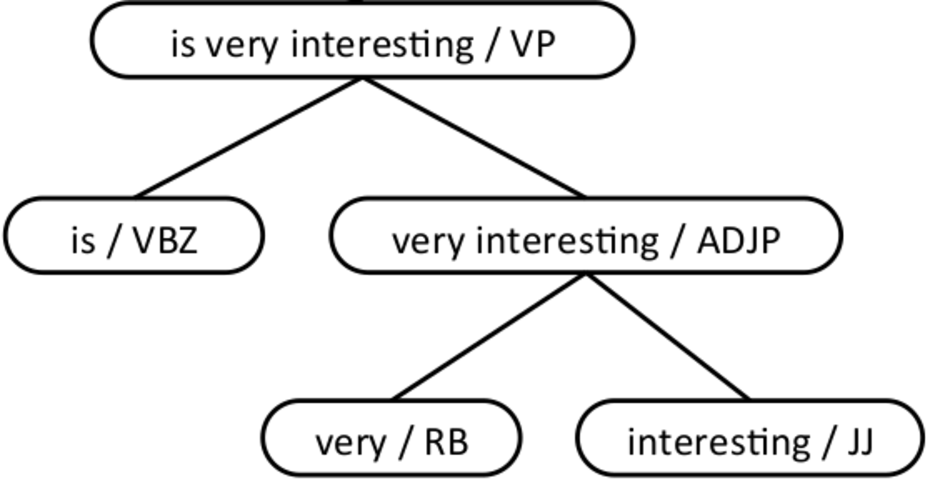
\includegraphics[scale=0.5]{figure/example-parse}
    \caption[Constituency parse tree for the phrase ``is very interesting'']{Constituency parse tree for the phrase ``is very interesting''.}
    \label{fig:example-parse}
\end{figure}

\begin{figure}[H]
    \centering
    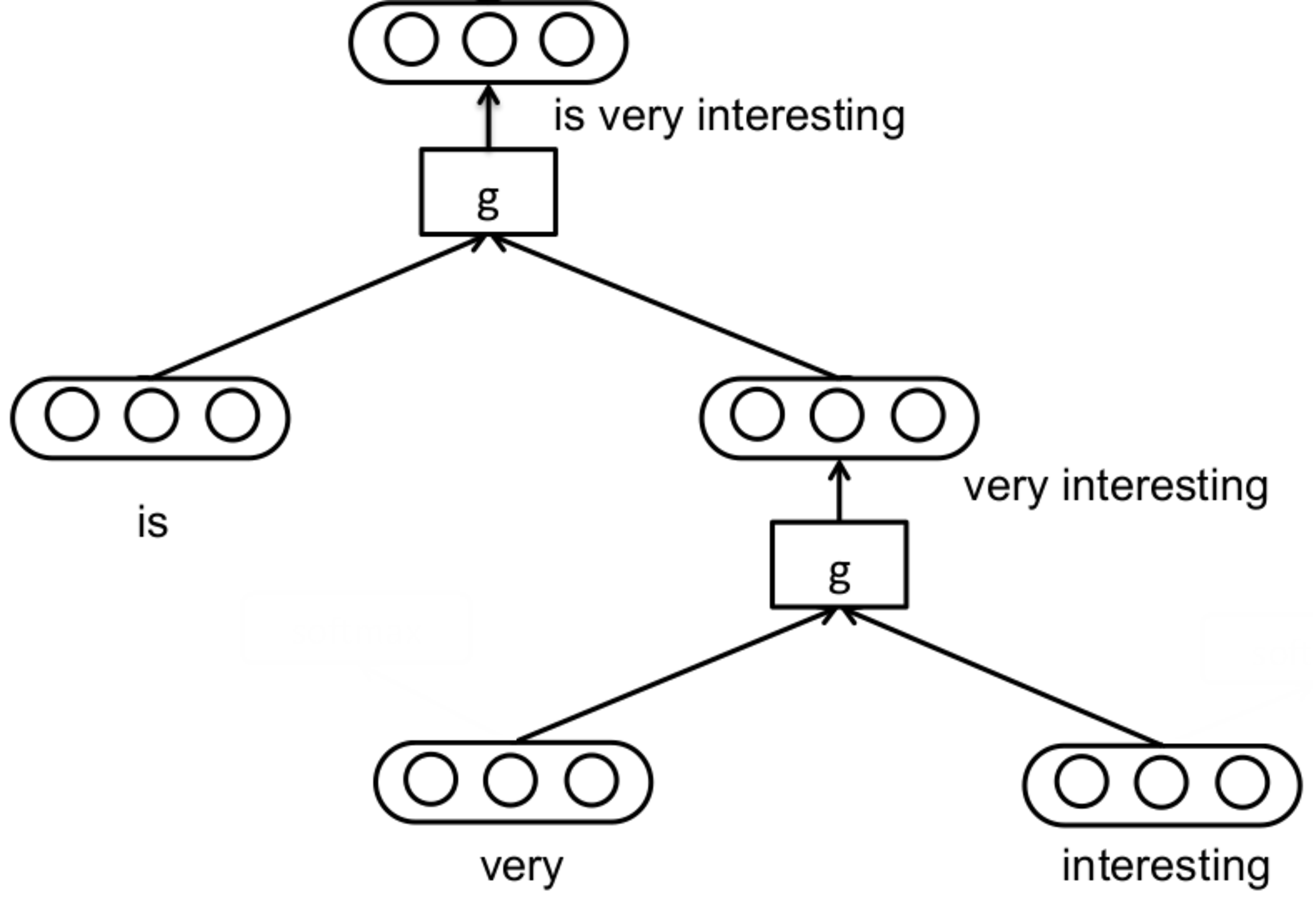
\includegraphics[scale=0.46]{figure/example-compose}
    \caption[Applying Recursive Neural Network on the phrase ``is very interesting'']{Applying Recursive Neural Network on the Constituency parse tree of the phrase ``is very interesting''.
    The composition function of this network is denoted as \textbf{g}.}
    \label{fig:example-compose}
\end{figure}

Recursive Neural Networks are linguistically attractive models due to their ability to compose sentences with respect to their parse trees~\cite{treeLSTM}.
Although having this ability, most Recursive Neural Networks (e.g. RNN, MV-RNN, RNTN~\cite{socher2013recursive}, DRNN~\cite{IrsoyDRNN}) do not explicitly utilize to local syntactic information at each parse tree's node.
By incorporating the local syntactic information into the composition function at each parse tree's node, TE-RNTN~\cite{tag-embedding-rnn} was able to not only dramatically improve the performance of RNTN (Socher, 2013)~\cite{socher2013recursive} (from \(85.4\%\) to \(87.7\%\) accuracy) but also their models used much smaller number of parameters \((54K)\) compared to that of RNTN \((108K)\)~\cite{tag-embedding-rnn}.
Composing process of the Constituency parse tree of the phrase ``is very interesting'' using TE-RNTN is illustrated in Fig.\ref{fig:example-compose-tag}.

\begin{figure}[H]
    \centering
    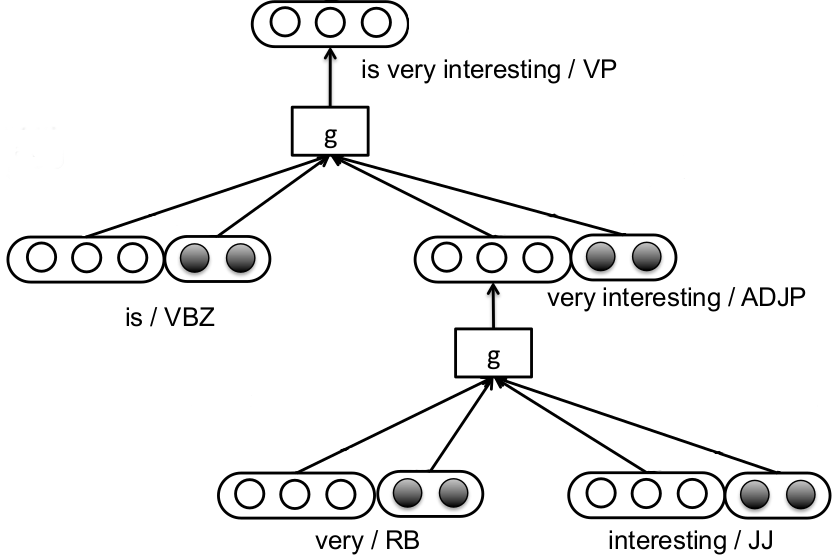
\includegraphics[scale=0.4]{figure/example-compose-tag}
    \caption[Applying TE-RNTN on the phrase ``is very interesting'']{Applying TE-RNTN~\cite{tag-embedding-rnn} on the Constituency parse tree of the phrase ``is very interesting''.
    The composition function of this network is denoted as \textbf{g}.
    To compose vector presentation of a phrase, composition function \textbf{g} takes vector presentations of: its constituting phrases (words); categories of the grammar of those phrases (words).}
    \label{fig:example-compose-tag}
\end{figure}

Shortly after the publication of TE-RNTN, Tree-LSTMs~\cite{treeLSTM} were introduced.
The core idea behind the design of Tree-LSTMs is to generalize the LSTMs for tree-structured inputs.
Tree-LSTMs were able to archive state-of-the-art performance on two tasks: predicting the semantic relatedness of two sentences (SemEval 2014, Task 1~\cite{SemeEvalTask1}) and sentiment classification (Stanford Sentiment Treebank~\cite{socher2013recursive}).
Despite thier successes, similar to RNTN~\cite{socher2013recursive}, Tree-LSTMs do not explicitly utilize to local syntactic information at each parse tree's node.

\subsubsection{Hypothesis}
Given the success of TE-RNTN, we hypothesized that by parameterized the composition functions of a Tree-LSTMs unit at a node with respect to the grammar rule expanding that node, we can improve the performance of Tree-LSTMs (in the same way how this method improving RNTN).

\subsubsection{Experiment}
We did experiments on several variations of Tree-LSTMs which incorporating different types local syntactic features.
These features includes Constituency grammar rule, Dependency relation, part-of-speech tag and a combination of both Dependency relation, part-of-speech tag.

One of our models was able to outperformed Dependency Tree-LSTM when using the same dependency parsed dataset.
But disappointedly, TE Tree-GRU underperformed Dependency Tree-LSTM on task of Semantic Relatedness (SemEval 2014, Task 1~\cite{SemeEvalTask1}) which pointed out the strength of Dependency Tree-LSTM and the main reason why it was presented in the original paper~\cite{treeLSTM}.
\textbf{In general, this approach was failed to improve Tree-LSTMs}, so we tried two more different approaches.

\subsection{Transfer Learning by retraining Glove on Amazon Reviews dataset}
\label{sec:second-method}
\subsubsection{Observation}
There are many words (e.g. ``B-rated'', ``Batman'', ``Nolan'', ``cartoonlike'') which rarely appears in regular documents but more often in movie reviews.
Additionally, the ways people use words in movie reviews might different from their usage in general documents.
For example the vector presentations of ``sympathy'' and ``disappointed'', or ``boom'' and ``insult'' are very close to each other in Glove Common Crawl\footnote{Common Crawl (840B tokens, 2.2M vocab, cased, 300d vectors, 2.03 GB download) publicly available at \url{https://nlp.stanford.edu/projects/glove/}} but if we have to predict the sentiment of a movie comment which has one of these word, they should be distinctive.

Noticeably, many experiments~\cite{treeLSTM}~\cite{KimCNN} have shown that modifying word embeddings during the training process help improving performance of Deep Learning systems.
Although this method helps to improve models' performance, it can harm generalization by updating only words which appear in the training set and not related words which only appear in test set.
We demonstrates a case in which this method harm the generalization ability of a classifier in Fig.\ref{fig:updating-word-bad-1} and Fig.\ref{fig:updating-word-bad-2}\footnote{Source: \url{https://cs224d.stanford.edu/lectures/CS224d-Lecture4.pdf}}.


\begin{figure}[H]
    \centering
    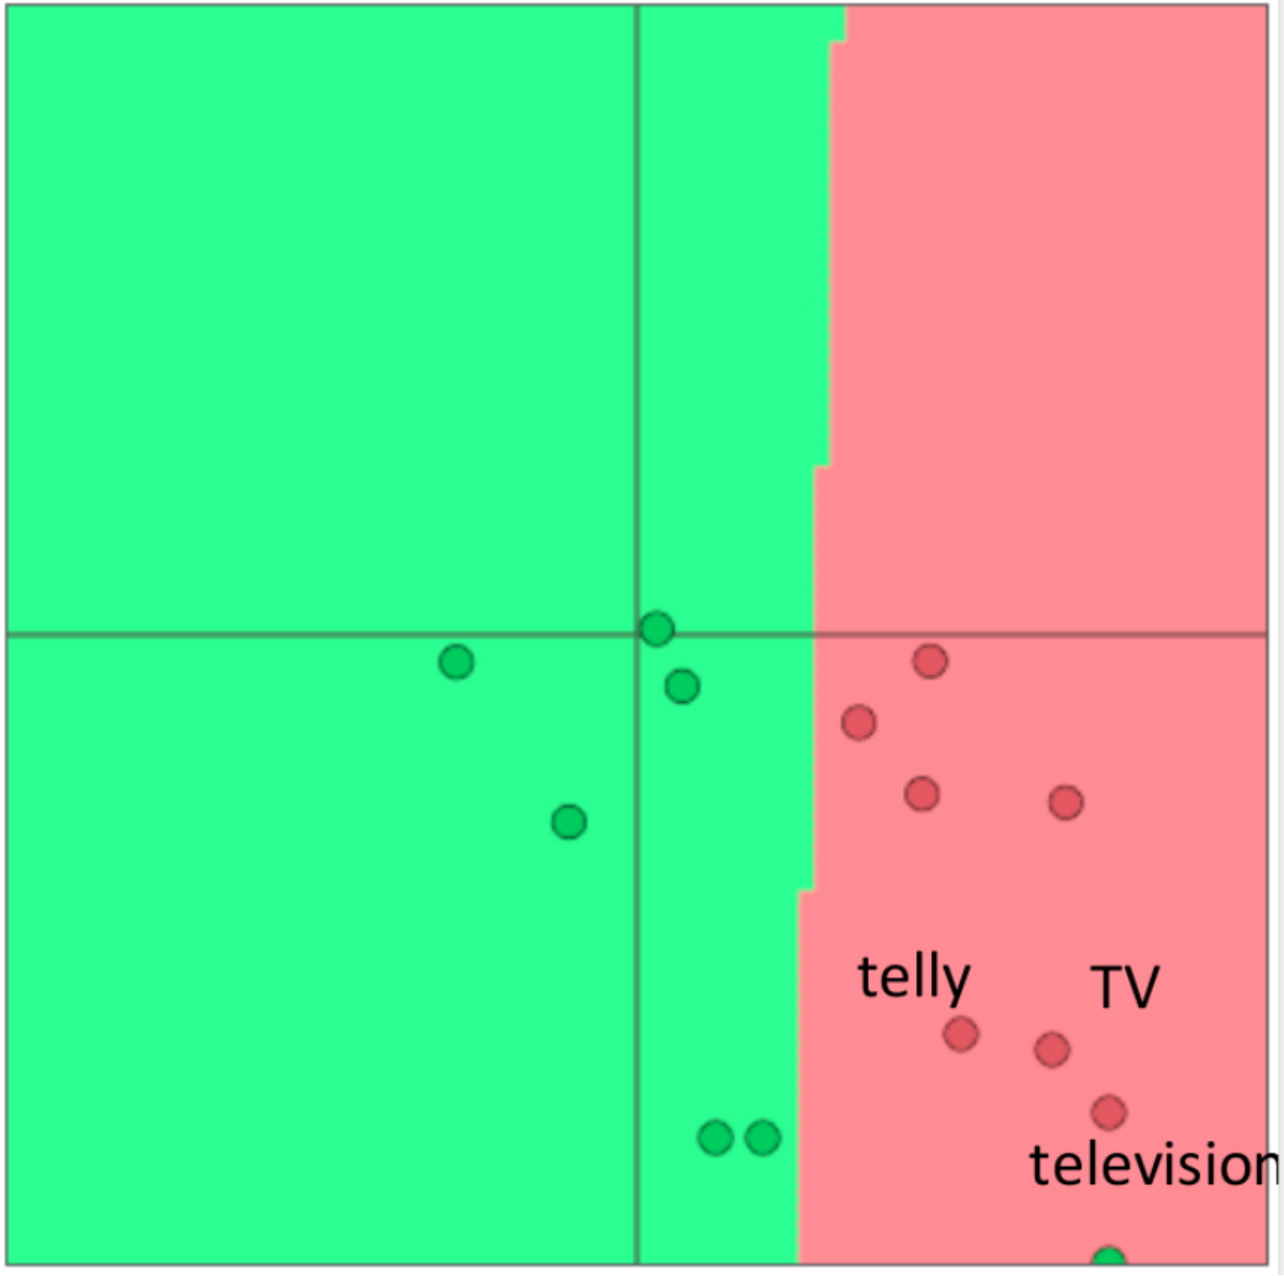
\includegraphics[scale=0.35]{figure/vec-before-update}
    \caption[Word embeddings updating causing over-fitting 1]{Vector presentations of words before being updated by the training process.
    Note that ``telly'', ``TV'' and ``television'' are still close to each other before being updated.
    The words ``telly'' and ``TV'' appear in the training set, but ``television'' does not.
    The green dot at the bottom right corner belong to training set, so the training process will "try" to fix this by updating vector presentations of ``telly'' and ``TV''.
     }
    \label{fig:updating-word-bad-1}
\end{figure}

\begin{figure}[H]
    \centering
    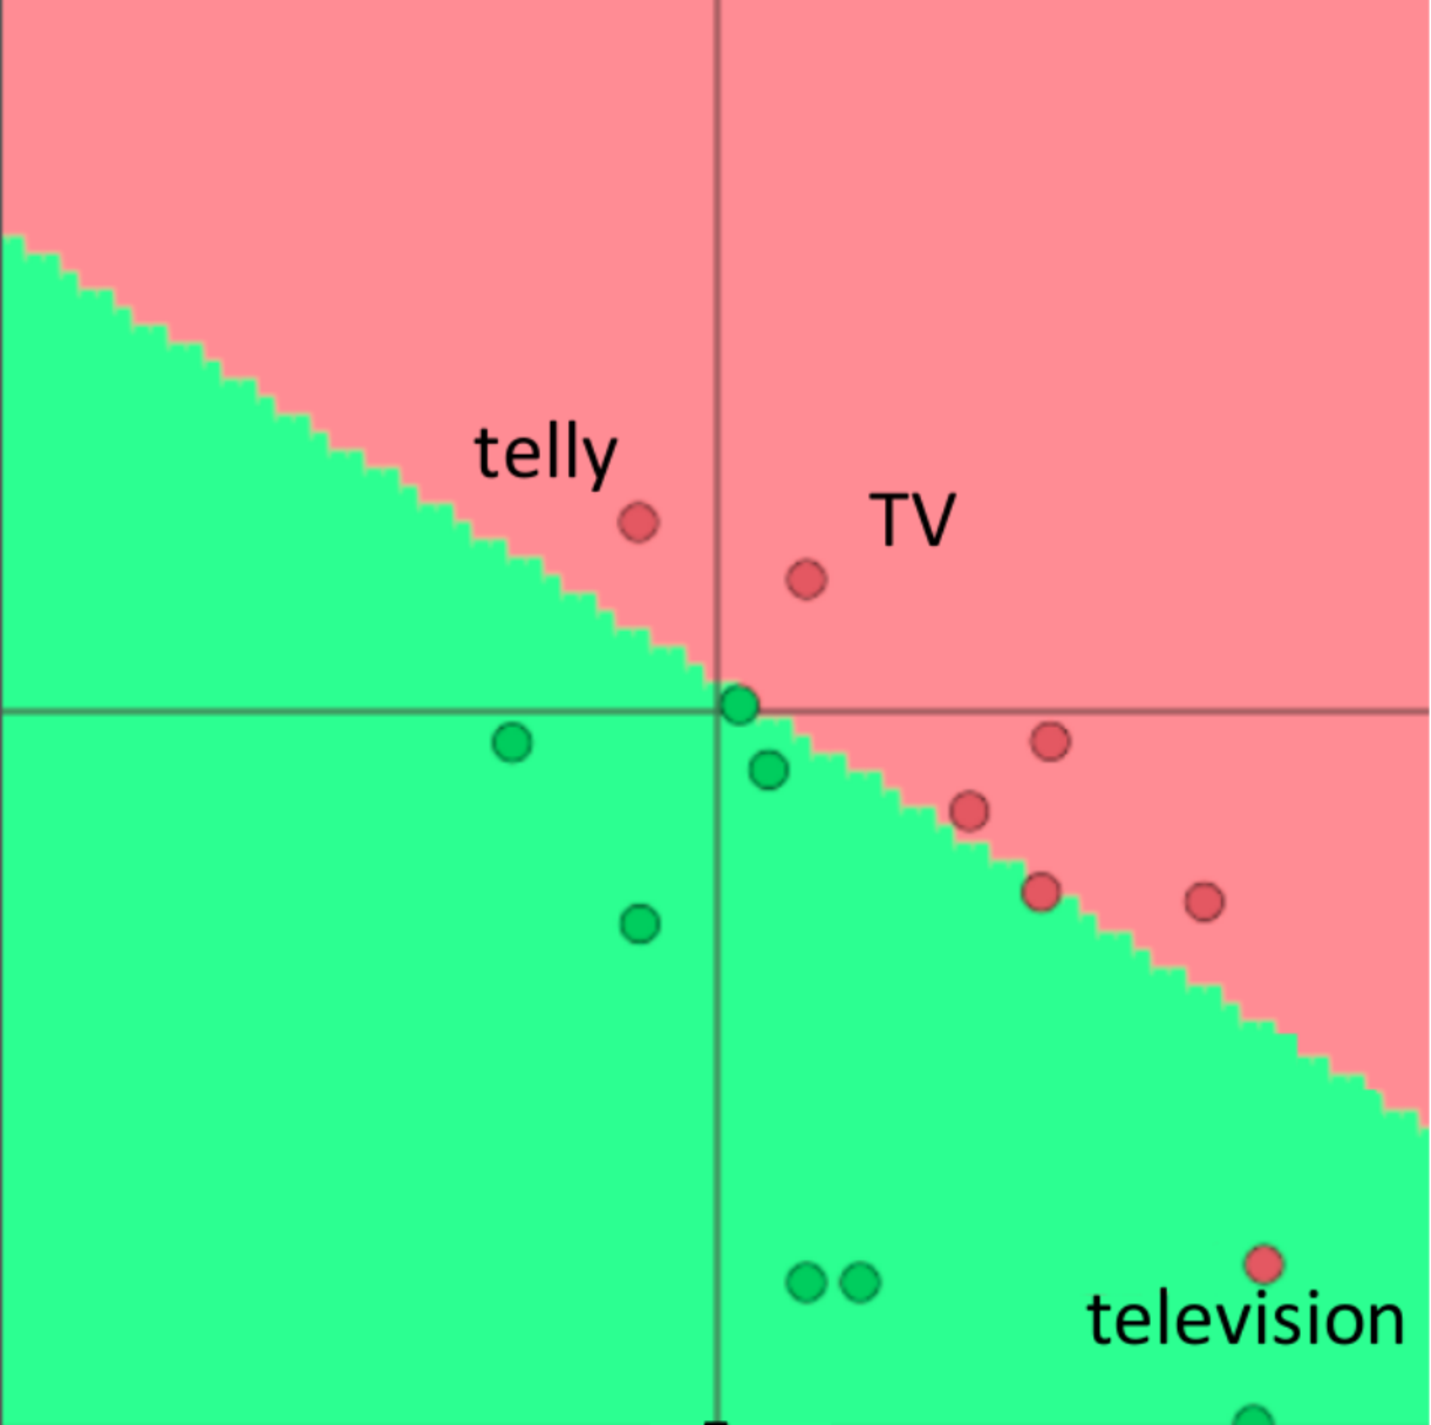
\includegraphics[scale=0.31]{figure/vec-after-update}
    \caption[Word embeddings updating causing over-fitting 2]{Vector presentations of words after being updated by the training process.
    In the test set, the trained classifier is likely to wrongly classify the examples which contain the word ``television''.}
    \label{fig:updating-word-bad-2}
\end{figure}

We also observe that the available amount of document-level labeled sentiment data (e.g. Amazon Reviews dataset~\cite{amazon-reviews} has 83.68 million reviews) is gigantic compared to the amount of sentence or phrase-level sentiment data (e.g. Stanford Sentiment Treebank~\cite{socher2013recursive} has 8544 sentences in its training set, even it is the biggest sentence-level sentiment analysis dataset).
Although, there are some attempts to do transfer learning~\cite{group-instance}~\cite{re-embedding} (i.e. training on large document-level sentiment dataset then fine-tuning and/or test on sentence-level sentiment dataset), their performances are not high when evaluated on Stanford Sentiment Treebank~\cite{group-instance}.

\subsubsection{Hypothesis}
We utilized Glove method to do transfer learning.
We hypothesized that by training Glove on review documents, especially movie or book reviews, we can capture more rare words and also the different way people use words (or different word relationships) to express their opinions on movies or books.
This might help our models archiving better generalisation when training on small sentence-level sentiment dataset like Stanford Sentiment Treebank.

\subsubsection{Experiment}
For archiving these purposes, we retrained Glove vectors~\cite{glove} on part of  \hyperref[sec:amazon]{Amazon Reviews dataset}.
This new Glove vectors was named \textbf{Glove Amazon}.
For evaluating Glove Amazon, we replaced the Glove Common Crawl\footnote{Common Crawl (840B tokens, 2.2M vocab, cased, 300d vectors, 2.03 GB download) publicly available at \url{https://nlp.stanford.edu/projects/glove/}} with Glove Amazon for initializing Tree-LSTMs' word embedding layer.

\textbf{In spite of being a simple method, it dramatically improves Tree-LSTMs performance.}
This is our first successful method for transfer learning from document-level (Amazon Reviews) to sentence-level labeled dataset (Stanford Sentiment Treebank).
Inspired by this method, we cooperated it into the development of our next approach.

\subsection{Combining Recusive Neural Networks with Convolution Neural Networks}

\subsubsection{Observation}
\paragraph{Convolution Neural Networks and Recusive Neural Networks}
Convolution Neural Networks (CNNs) have been proven to be effective models for the task of sentence-level sentiment analysis~\cite{KimCNN}.
Although being a simple Convolution Neural Network architect on top of pre-trained word embedding channels, CNN-multichannel~\cite{KimCNN} was able to archive state-of-the-art performance\footnote{2014} on Stanford Sentiment Treebank with binary setting.
Despite its success, for dealing with the problem composing fixed size presentation vectors given variable-length input sentences, CNN-multichannel utilized max-over-time pooling layer~\cite{nlp-scratch}.
\textbf{Although max-over-time pooling largely simplified the network (which is good for preventing over-fit), this solution have a clear drawback: the vector presentation of a sentence only tell if a feature appears in the sentence or not, the information about position of the feature is ignored}.
The structure of CNN-multichannel is demonstrated in Fig.\ref{fig:CNN-multichannel}~\cite{KimCNN}.

\begin{figure}[H]
    \centering
    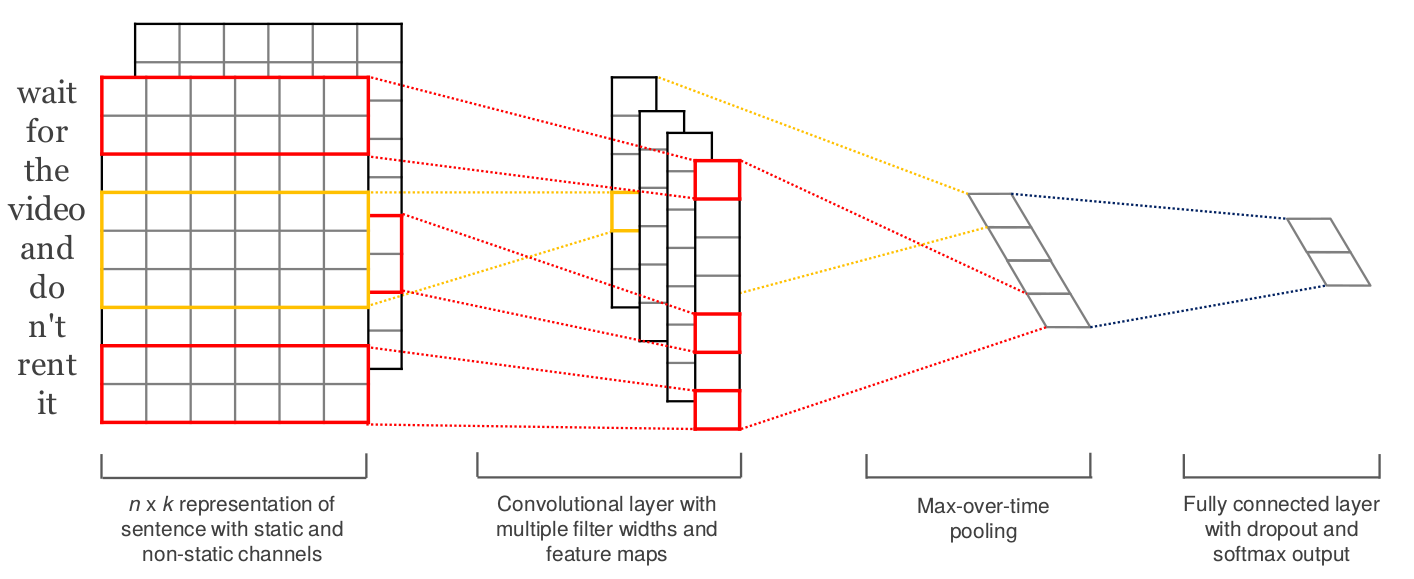
\includegraphics[scale=0.33]{figure/sentencecnn}
    \caption[CNN-multichannel]{Structure of CNN-multichannel. 
    At the convolution layer, each filter produces a feature map of the input sentence. 
    In turn, each feature map through the max-over-time pooling layer produces a feature in the vector presentation of the sentence}
    \label{fig:CNN-multichannel}
\end{figure}

For dealing with the problem composing fixed size presentation vectors given variable-length input sentences, one intuitive solutions would be to apply Recurrent Neural Networks~\cite{cnn-rnn}.
Another more complicated solution is utilizing Recursive Neural Networks.
\textbf{Recursive Neural Networks have several advantages over Recurrent Neural Networks}~\cite{need-tree}~\cite{bowman-treevslstm}: 
\begin{itemize}
\item In case the input sequence belongs to recursively defined language, given only a small subset of the data with limited length sentences, tree structures model have better ability to generalize compare to sequential ones.
But when we increase the limited length sentences, the advantage of tree over sequential models decrease fast~\cite{bowman-treevslstm}. 
\item Tree can breaks down complicated sentences into simpler phrases, which make it easier for generalization~\cite{knowledge-matter}~\cite{need-tree}.
\item Some features which are far apart when a sentence is presented as sequence become closer when it is presented as tree~\cite{need-tree}.
\end{itemize}

\textbf{Tree-LSTMs also have some drawbacks}, these drawbacks including:
\begin{itemize}
\item Sentences can be wrongly parsed, especially when comments are expressed in informal language.
The performance of the system depends on the parser being used.
\item At their leaf-module, Tree-LSTMs have only a simple logistic regression layer on top of the vector presentation of a single word at that position (Sec.\ref{sec:treelstm}). 
\end{itemize}

\paragraph{Language Modeling}
After the success of the second approach (Transfer Learning by retraining Glove on Amazon Reviews dataset (Sec.\ref{sec:second-method})), we want to do more experiments with Transfer Learning methods.
In Glove method~\cite{glove}, the meaning of words are captured by encoding the ratios between their co-occurrence probabilities.
Different from Glove method, by pre-training a model as Language Model, the model learns to predict the words given their left context.
Additionally, this pre-training method give us the ability to pre-train the entire model, not just the word embeddings. 
Language Modeling pre-training method has been reported~\cite{semisup-seq2seq} to dramatically improve accuracy of LSTMs on Rotten Tomatoes sentiment classification dataset~\cite{Rotten-Tomato} (which is a super set of Stanford Sentiment Treebank data set).

\subsubsection{Hypothesis}
\paragraph{Convolution Neural Networks and Recusive Neural Networks}
The simple leaf-module of Tree-LSTMs might its weakness when dealing with the problem of words ambiguity.
This weakness becomes even more severe when the sentence is wrongly parsed.
Different from Tree-LSTMs, CNN-multichannel's~\cite{KimCNN} first convolution layer have hundred of filters, each produces a feature map of the sentence by sliding through it with window sizes 3 to 5 words.
Filters with large context window help CNN-multichannel to mitigate the problem of words ambiguity and to capture phrase-level feature.
We think this is the reason why CNN-multichannel  can outperform TreeLSTMs, even when it have no respect for the positions of features. 

We combined Convolution Neural Networks with Tree-LSTM and sequential LSTM.
We hypothesized that the convolution layer will help Tree-LSTMs to mitigate the problem of lacking local context and words ambiguity at leaf nodes.
Additionally, using Tree-LSTM to combine the feature maps produced by the convolution layer might be a better choice compared to using max-over-time pooling layer.
\paragraph{Language Modeling}
The increased model complexity can lead to over-fitting.
We tackled this risk by unsupervised pre-training the models on the large Amazon Reviews dataset using methods described in Sec.\ref{sec:unsupervised-pretrain}.
If we pre-train our models on part of Amazon Reviews dataset, we hypothesized this pre-training method offers these benefits:
\begin{itemize}
\item In many cases, words or phrases have different meaning depend on their contexts (e.g. when words are used to composed idioms, these idioms cannot be understood if taken literally).
These information about how to compose words can be embedded in word embeddings or parameters of the model.
\item By training Language Model on part of Amazon Reviews dataset, we also want the model to learn more specific dependencies: The reviewer cries when watching a good romantic movie, or the viewer praises the novel and then criticizes the movie based on how good the novel is, or how sentiments being affected by sentence structures. 
\end{itemize} 

\subsubsection{Experiment}
For this approach, we do experiment with two network architects:
\begin{description}
\item[CNN Tree-LSTM] We inserted a convolution layer between the word embedding layer and the Tree-LSTM's leaf-module.
The rest of TreeLSTM implementation was kept unchanged.

\item[CNN LSTM] Similar CNN Tree-LSTM but the Tree-LSTM module is replaced by sequential LSTM\footnote{Although CNN LSTM seems similar to \hyperref[cnn-rnn]{CNN-RNN}~\cite{cnn-rnn}, we extended it for multichannel input and unsupervised pre-train it.}
One advantage of CNN-LSTM compared to CNN Tree-LSTM is that CNN-LSTM can be unsupervised pre-trained as Language Model, while CNN Tree-LSTM can not (Sec.\ref{sec:unsupervised-pretrain}).
\end{description}

With this approach, \textbf{we was able to archive state-of-art\footnote{July, 2017} performance on Stanford Sentiment Treebank}.


\section{Contributions}
In search of new improvements on the task of sentence-level sentiment analysis, we have tried three approaches: Utilizing local syntactic information at each node of Recursive Neural Networks; Transfer Learning by retraining Glove on Amazon Reviews dataset and Combining Recursive Neural Networks with Convolution Neural Networks.
Based on our experiments, we conclude that:
\begin{itemize}
\item Glove Amazon significantly improves the original Tree-LSTMs with Glove Common Crawl word embeddings.

\item For sentiment analysis on movie reviews, our experiment results support the existence of useful features in Glove Amazon which does not exist or hardly be extracted in Glove Common Crawl.
On the other hand, there also exist useful features that does not appear in Glove Amazon but only appear in Glove Common Crawl or when combining both Glove Amazon and Glove Common Crawl.

\item By adding a convolution layer before the leaf-node of Tree-LSTM, the performance of Tree-LSTM was dramatically improved.
The new model was named CNN Tree-LSTM. 
With help from Glove Amazon word embeddings, CNN Tree-LSTM was able to reach state-of-the-art performance.

\item  Tree-LSTMs have already utilized the information in word embeddings and the local syntactic information from tag embeddings adding no more value.
\end{itemize}

\section{Structure of this thesis}
\begin{description}
\item [\deschyperlink{chap:background}{Chapter 2}] introduces some basic knowledge in NLP, Deep Learning and programming framework for implementing Deep Learning systems.
\item [\deschyperlink{chap:related}{Chapter 3}] builds up the theoretical framework for the whole thesis.
It analyzes the closely related works -- all the models or methods presented here are being used by at least one of our models.
For clarity, we divide Chapter 3 into three parts.
The first part is \hyperref[sec:dataset]{"Datasets"}.
This part contains information about all datasets which were used in this thesis.
The second part is \hyperref[sec:composer]{"Neural network architects for sentence composition"}.
The models presented in this part are used to compose vector presentations of sentences.
These presentation vectors are then used to classify the sentiment class of the sentence.
For each model, we describe its structure, training method and evaluation on SST.
Additionally, we analyze advantages and disadvantages of each model compared to the others.
In the last part, we present and discuss several \hyperref[sec:unsupervised-pretrain]{unsupervised pre-train methods}.
\item [\deschyperlink{chap:method}{Chapter 4}] describes our new network architects, the reasons behind their designs, their training methods and other experiments.
\item [\deschyperlink{chap:result}{Chapter 5}] presents, analyzes and discusses the empirical comparisons of our models and other related models.
\item [\deschyperlink{chap:conclude}{Chapter 6}] summarizes the achieved results, describes future works and conclusion.
\end{description}
